\documentclass{beamer}
\usepackage[utf8]{inputenc}

\usetheme{Madrid}
\usecolortheme{default}
\usepackage{amsmath,amssymb,amsfonts,amsthm}
\usepackage{txfonts}
\usepackage{tkz-euclide}
\usepackage{listings}
\usepackage{adjustbox}
\usepackage{array}
\usepackage{tabularx}
\usepackage{gvv}
\usepackage{lmodern}
\usepackage{circuitikz}
\usepackage{tikz}
\usepackage{graphicx}

\setbeamertemplate{page number in head/foot}[totalframenumber]

\usepackage{tcolorbox}
\tcbuselibrary{minted,breakable,xparse,skins}



\definecolor{bg}{gray}{0.95}
\DeclareTCBListing{mintedbox}{O{}m!O{}}{%
	breakable=true,
	listing engine=minted,
	listing only,
	minted language=#2,
	minted style=default,
	minted options={%
		linenos,
		gobble=0,
		breaklines=true,
		breakafter=,,
		fontsize=\small,
		numbersep=8pt,
		#1},
	boxsep=0pt,
	left skip=0pt,
	right skip=0pt,
	left=25pt,
	right=0pt,
	top=3pt,
	bottom=3pt,
	arc=5pt,
	leftrule=0pt,
	rightrule=0pt,
	bottomrule=2pt,
	toprule=2pt,
	colback=bg,
	colframe=orange!70,
	enhanced,
	overlay={%
		\begin{tcbclipinterior}
			\fill[orange!20!white] (frame.south west) rectangle ([xshift=20pt]frame.north west);
	\end{tcbclipinterior}},
	#3,
}
\lstset{
	language=C,
	basicstyle=\ttfamily\small,
	keywordstyle=\color{blue},
	stringstyle=\color{orange},
	commentstyle=\color{green!60!black},
	numbers=left,
	numberstyle=\tiny\color{gray},
	breaklines=true,
	showstringspaces=false,
}
%------------------------------------------------------------
%This block of code defines the information to appear in the
%Title page
\title %optional
{1.5.35}
\date{}
%\subtitle{A short story}

\author % (optional)
{Revanth Siva Kumar D- EE25BTECH11048}



\begin{document}
	
		\frame{\titlepage}
	\begin{frame}{Question}\textbf{Question}:The mid-point of segment $AB$ is the point $P(0,4)$. If the coordinates of $B$ are $(-2,3)$ then the coordinates of $A$ are \underline{\hspace{1.5cm}}.
    \end{frame}

\begin{frame}{Theoretical Solution}
    \textbf{Given Information}  

The midpoint of segment $AB$ is $P(0,4)$.  

The coordinates of point $B$ are $(-2,3)$.  

We need to find the coordinates of point $A$ using a specific matrix method based on the section formula.  


\textbf{Matrix Setup}  

First, write the coordinates of the points as column matrices:  

\begin{align*}
    P = \myvec{0 \\ 4}, 
\end{align*}
\begin{align*}
    B = \myvec{-2 \\ 3}, 
\end{align*}
\begin{align*}
    A = \myvec{x \\ y}
\end{align*}
\end{frame}
\begin{frame}{Theoretical Solution}
    \textbf{The Formula}  

Since $P$ is the midpoint, it is known that $A$ divides $BP$ in the ratio -2:1 internally or in other words 2:1 externally.
Here k = -2, Thus by section formula:
\begin{align*}
A = \frac{kP+B}{1+k}
\end{align*}
Substituting k = -2 we get
\begin{align*}
    A = 2P - B
\end{align*}


\textbf{Calculation}  

Substitute the matrices:  
\begin{align*}
    A = 2 \myvec{0 \\ 4} - \myvec{-2 \\ 3}
\end{align*}



Scalar multiplication:  
\begin{align*}
    A = \myvec{0 \\ 8} - \myvec{-2 \\ 3}
\end{align*}
\end{frame}
\begin{frame}{Theoretical Solution}
    Matrix subtraction:  
\begin{align*}
A = \myvec{0 - (-2) \\ 8 - 3} 
= \myvec{2 \\ 5}    
\end{align*}



\textbf{Conclusion} 

The coordinates of point $A$ are $(2,5)$.  

Quick check: midpoint of $A(2,5)$ and $B(-2,3)$ is  
\begin{align*}
    \left(\frac{2+(-2)}{2}, \frac{5+3}{2}\right) = (0,4) = P
\end{align*}
\end{frame}

\begin{frame}[fragile]
\frametitle{C Code - Section formula function}
\begin{lstlisting}
#include <stdio.h>

void findA(int xp, int yp, int xb, int yb, int *xa, int *ya) {
    *xa = 2*xp - xb;
    *ya = 2*yp - yb;
}
\end{lstlisting}
\end{frame}

\begin{frame}[fragile]
	\frametitle{Python Code through shared output}
	\begin{lstlisting}
import ctypes
import numpy as np
import matplotlib.pyplot as plt

# Load the compiled C library
lib = ctypes.CDLL("./findA.so")

# Define the function signature: void findA(int, int, int, int, int*, int*)
lib.findA.argtypes = [
    ctypes.c_int, ctypes.c_int,
    ctypes.c_int, ctypes.c_int,
    ctypes.POINTER(ctypes.c_int),
    ctypes.POINTER(ctypes.c_int)
]
lib.findA.restype = None  # void
\end{lstlisting}
\end{frame}

\begin{frame}[fragile]
\frametitle{Python Code through shared output}
\begin{lstlisting}
def findA(xp, yp, xb, yb):
    """Call the C function via ctypes."""
    xa = ctypes.c_int()
    ya = ctypes.c_int()
    lib.findA(xp, yp, xb, yb, ctypes.byref(xa), ctypes.byref(ya))
    return xa.value, ya.value
    
if __name__ == "__main__":
    xp, yp = 3, 4
    xb, yb = 1, 2

    xa, ya = findA(xp, yp, xb, yb)
    print(f"Coordinates of A (from C): ({xa}, {ya})")

\end{lstlisting}
\end{frame}
\begin{frame}[fragile]
	\frametitle{Python Code through shared output}
	\begin{lstlisting}
	# Plotting
    plt.figure(figsize=(6, 6))
    plt.plot(xp, yp, 'ro', label='P')
    plt.plot(xb, yb, 'bo', label='B')
    plt.plot(xa, ya, 'go', label='A')
    plt.plot([xb, xa], [yb, ya], 'k--', label='Line BA')

    plt.text(xp+0.1, yp+0.1, "P")
    plt.text(xb+0.1, yb+0.1, "B")
    plt.text(xa+0.1, ya+0.1, "A")

    plt.axhline(0, color='black', linewidth=0.5)
    plt.axvline(0, color='black', linewidth=0.5)
    plt.grid(True)
    plt.legend()
    plt.title("Reflection of B across P (computed by C, plotted by Python)")
    plt.show()
	
	\end{lstlisting}
\end{frame}

\begin{frame}[fragile]
	\frametitle{Python code : Direct }
	
	\begin{lstlisting}

import sys                                        
import numpy as np
import numpy.linalg as LA
import matplotlib.pyplot as plt
import matplotlib.image as mpimg

#local imports
from libs.line.funcs import *
from libs.triangle.funcs import *
from libs.conics.funcs import circ_gen


#if using termux
import subprocess
import shlex
#end if
\end{lstlisting}
\end{frame}
\begin{frame}[fragile]
	\frametitle{Python code : Direct }
	
	\begin{lstlisting}

#Given points
P = np.array(([0,4])).reshape(-1,1)
B = np.array(([-2,3])).reshape(-1,1)

#Ratio
n=-2/1

#Point
A= (B+n*P)/(1+n) # calculating the coordinate points of R which divides the join between the two points
#print(R)

#Generating all lines
x_PB = line_gen(A,B)

#Plotting all lines
plt.plot(x_PB[0,:],x_PB[1,:],label='$PB$')
\end{lstlisting}
\end{frame}
\begin{frame}[fragile]
	\frametitle{Python code : Direct }
	
	\begin{lstlisting}

#Labeling the coordinates
tri_coords = np.block([[P,B,A]])
plt.scatter(tri_coords[0,:], tri_coords[1,:])
vert_labels = ['P','B','A']
for i, txt in enumerate(vert_labels):
    #plt.annotate(txt, # this is the text
    plt.annotate(f'{txt}\n({tri_coords[0,i]:.0f}, {tri_coords[1,i]:.0f})',
                 (tri_coords[0,i], tri_coords[1,i]), # this is the point to label
                 textcoords="offset points", # how to position the text
                 xytext=(20,-10), # distance from text to points (x,y)
                 ha='center') # horizontal alignment can be left, right or center
# use set_position
\end{lstlisting}
\end{frame}
\begin{frame}[fragile]
	\frametitle{Python code : Direct }
	
	\begin{lstlisting}

ax = plt.gca()
#ax.spines['top'].set_color('none')
#ax.spines['left'].set_position('zero')
#ax.spines['right'].set_color('none')
#ax.spines['bottom'].set_position('zero')
ax.spines['left'].set_visible(False)
ax.spines['right'].set_visible(False)
ax.spines['top'].set_visible(False)
ax.spines['bottom'].set_visible(False)
#plt.xlabel('$x$')
#plt.ylabel('$y$')
plt.legend(loc='best')
plt.grid() # minor
plt.axis('equal')
plt.show()
 \end{lstlisting}

 \end{frame}

\begin{frame}{Plot by python using shared output from c}
	\begin{center}
		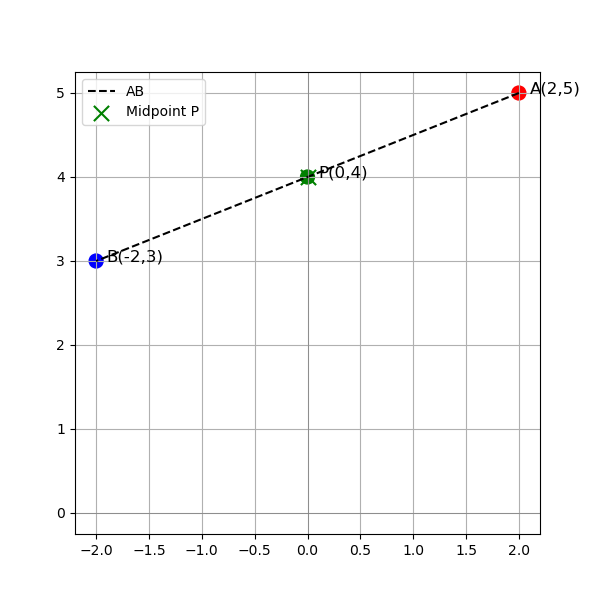
\includegraphics[width=0.6\columnwidth]{figs/Figure_2.png}
	\end{center}
\end{frame}


\begin{frame}{Plot by python using shared output from c}
	\begin{center}
		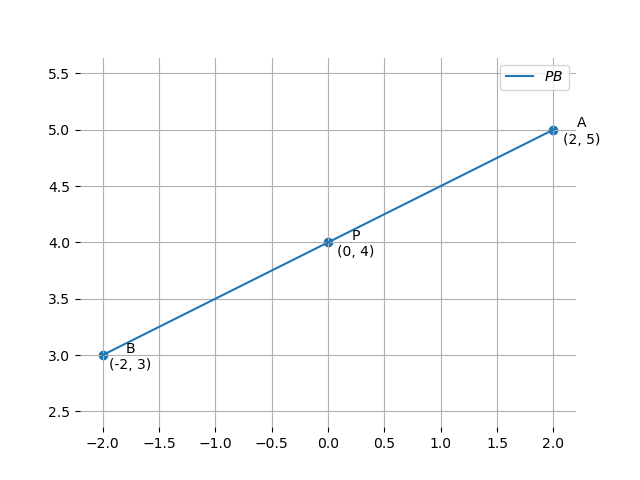
\includegraphics[width=0.6\columnwidth]{figs/Figure_1.png}
	\end{center}
\end{frame}
\end{document}
